\section{Introduction}
This chapter of the report details the experimental approach taken when developing the systems responsible for the two main modes of (Navigation and Detail).

Each mode has differing functionality, but shares some common components --- the specifics of these components have been detailed in section \ref{sec:sharedcomponents}.   

\section{Technical Background}
\subsection{Languages}
A majority of the development work done over the course of this project has been in Matlab, although Java and C++ have also been used.

\subsubsection{Matlab}
It was decided that Matlab was the right tool for the job for several reasons.

Firstly, Matlab has a lot of relevant functionality ``baked-in'' - for instance, an \ac{FFT} can be performed on a vector in one line: \lstinline$fft(vector)$, with no additional libraries required. This is not the case with many other languages. This makes prototyping much quicker, as it is not necessary to totally re-invent the wheel when trying new ideas.

Wrappers for OpenNI are available for Matlab, making interaction with the Xtion camera - the wrapper is open-source, so any modifications can be made quite easily.

Another major factor in choosing Matlab over another language is the amount of support available, both physically from my Project Supervisor, and online from the Matlab community. 

The project has been developed using Matlab r2014a, although should be backwards-compatible with most recent releases. 

\subsubsection{Java}
As large parts of Matlab run in the \ac{JVM}, it is possible to use Java classes directly from within Matlab. This was taken advantage of in order to use threads, which is something that Matlab does not support out of the box. 

Matlab r2014a runs under the Java JVM version 1.7 - as such, any development must be done using the Java 7 JDK or below. 

\subsubsection{C/C++}
C/C++ functions can be exported to the Matlab environment through the use of MEX-files. The OpenNI wrapper used to interact with the Xtion camera was written using C++ and MEX, and required some modifications.

Additionally, a C++ based Video Segmentation~\cite{videosegment} tool written by Google and Georgia Tech was trialled, and was also slightly modified.

\subsection{Data Acquisition}
The Asus Xtion Pro Live~\cite{xtion} camera used in this project is compatible with OpenNI, a framework used for developing ``Natural Interaction'' software.

A module available on the Matlab File Exchange~\cite{matlabwrapper} providers a wrapper for OpenNI, allowing the image and depth information to be retrieved from the camera.

Once compiled, the wrapper provides the following functions: \texttt{mxNiCreateContext}, \texttt{mxNiDeleteContext}, \texttt{mxNiPhoto} and \texttt{mxNiDepth}.

\begin{itemize}
    \item \texttt{mxNiCreateContext()} initialises the camera and returns a handle to the Xtion device.
    \item \texttt{mxNiPhoto(handles)} returns the current \ac{RGB} from the device referenced at \texttt{handles}.
    \item \texttt{mxNiPhoto(handles)} returns the current \ac{RGB} from the device referenced at \texttt{handles}.
    \item \texttt{mxNiDeleteContext(handles)} closes the connection to the camera 
\end{itemize}

Combining these methods, a basic Matlab program to acquire and display the RGB and Depth data from the camera as follows: 

\begin{lstlisting}[caption = {Acquiring Depth and RGB in Matlab}]
    handles = mxNiCreateContext();
    rgb = mxNiPhoto(handles);
    rgb = permute(rgb, [3 2 1]);
    depth = mxNiDepth(handles);
    depth = permute(depth, [2 1]);

    subplot(1, 2, 1);
    imshow(rgb);

    subplot(1, 2, 2);
    imshow(depth);
    colormap(jet);
\end{lstlisting}

The calls to \texttt{permute()} are necessary as the OpenNI wrapper returns the data in the opposite order to what Matlab expects.

By default, both \texttt{mxNiPhoto()} and \texttt{mxNiDepth()} return $320\times240$ images.

The data returned by \texttt{mxNiPhoto()} is a 3-channel image containing 8-bit integer intensity values for the Red, Green and Blue channels.
The data returned by \texttt{mxNiDepth()} is takes the form of a matrix of distance values, measured in millimeters.

\section{Navigation Mode}
As mentioned, the main focus of the Navigational of the system is to allow a user to walk around a room and avoid obstacles. Several prototype systems have been developed, each using different techniques to convey different data to the user.

\subsection{Central Distance}
\label{sec:centraldistance}
\subsubsection{Description}
It is possible to read the distance to the center of the image with the following code:

\begin{minted}{matlab}
    handles = mxNiCreateContext();
    rgb = mxNiPhoto(handles);
    rgb = permute(rgb, [3 2 1]);
    depth = mxNiDepth(handles);
    depth = permute(depth, [2 1]);
    
    centralDistance = depth(size(depth, 1), size(depth, 2));
\end{minted}


Building on this basic idea, a way of conveying this distance was developed. By synthesising a sine-wave with a varying frequency (from low to high) according to distance to the central point, and playing it back in real-time, a user could get a live idea of the distance to the object directly in front of them. As the minimum depth supported by the Xtion is around 550mm, and the maximum is around 4m (4000mm), a direct mapping from distance (in millimeters) to frequency (in Hertz) was used - these frequencies are well within the audible range of the human ear~\cite{hearingrange}.

\begin{figure}[H]
\centering
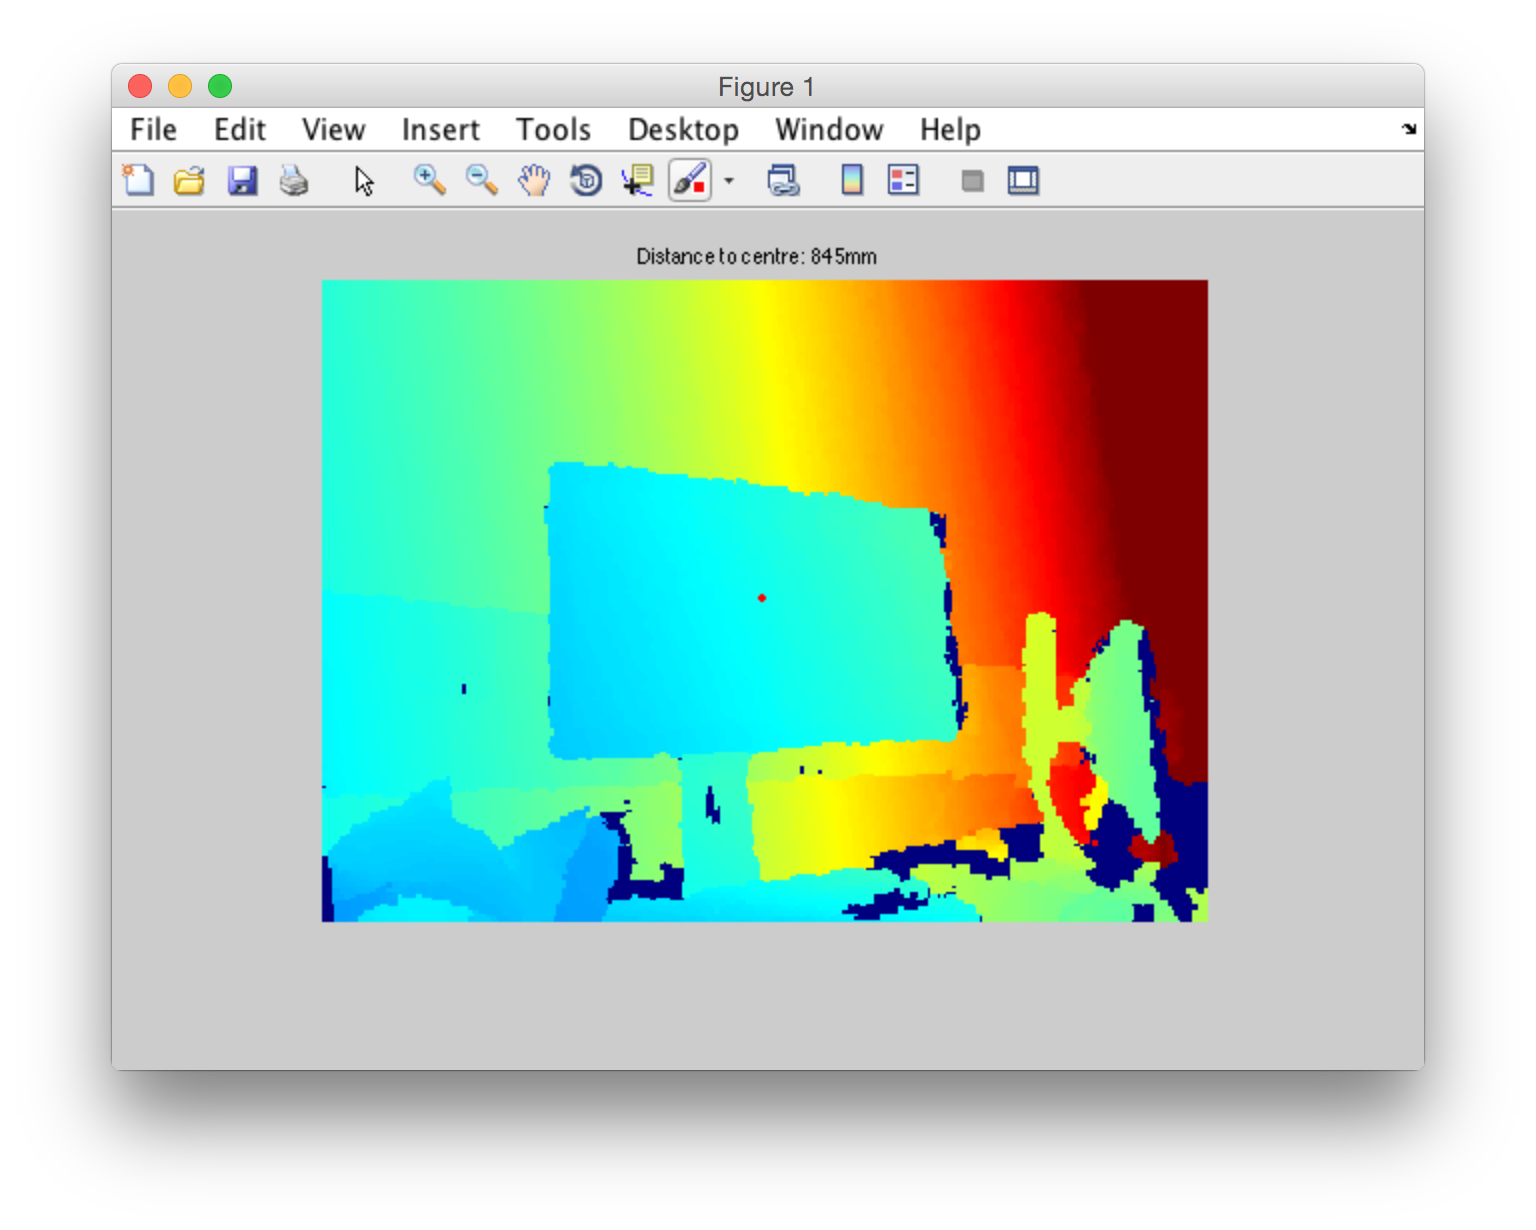
\includegraphics[width=0.6\textwidth]{Navigation/single-tone.png}
\caption{Variable-frequency distance system. The red dot marks the center of the depth map}
\end{figure}

This required the development of the tone-generation Java class detailed in \ref{sec:tonegen}, and the source-code for this prototype can be found in the file centralTone.m.

\subsubsection{System Performance}
As the algorithm is quite straight-forward, the software implementing it was not excessively CPU intensive. Measuring the performance of the script gave estimates that it performed at roughly 30Hz --- this limitation was probably due to the overhead of displaying the image of the depth map using \texttt{imshow()}, which was only being done for development purposes.

\subsubsection{Effectiveness}
The system was tested by walking around a room blindfolded, using only the camera to avoid obstacles. The test was a success --- the mapping from frequency to distance was quite intuitive, and there were no ``crashes'', in terms of both software and the physical sense.

However, I felt that the amount of information being sent to the user of the system could be improved. Given the range of possible frequencies (550-4000), the pitch resolution of the human auditory system (said to be around 1Hz~\cite{pitchres}), and the processing rate of the video feed, it is possible to get an approximation of the bitrate of the system:

\begin{equation}
\log _2\left({depth}_{max} - {depth}_{min}\right) \times 30 \approx 350 \mbox{bits/sec}
\end{equation}

\subsection{Central Distance with Size}
\subsubsection{Description}
Using the 350 bits/sec figure obtained from the entropy calculations in section \ref{sec:centraldistance} as the base-line to be improved upon, it was decided that additional information could be conveyed.

It was determined experimentally that knowing the size of the object in-front of the user was relevant --- with this information, the user knows by how much their will need to alter their trajectory to avoid hitting the object. 

It is possible to calculate the physical width and height of the field-of-view using the following formulae:

\begin{equation}
{FOV}_{width} = 2 \times d \times \tan\frac{58\degree}{2}
\end{equation}
\begin{equation}
{FOV}_{height} = 2 \times d \times \tan\frac{45\degree}{2}
\end{equation}

Where 58\degree  and 45\degree  are the horizontal and vertical \ac{FOV} of the Xtion camera respectively~\cite{xtion-spec}. 

This information alone is no more useful to for navigational purposes than the distance to central point - however, by extracting the object at the center of the image, and determining how much of the \ac{FOV} it occupies, it is possible to calculate the area of the object.

Using the Magic Wand extraction technique described in section \ref{sec:magicwand}, the central object was extracted as a binary image, where pixels marked 1 indicated that they were part of the object, and pixels marked 0 indicated that they were not. 
\begin{figure}[H]
    \centering
    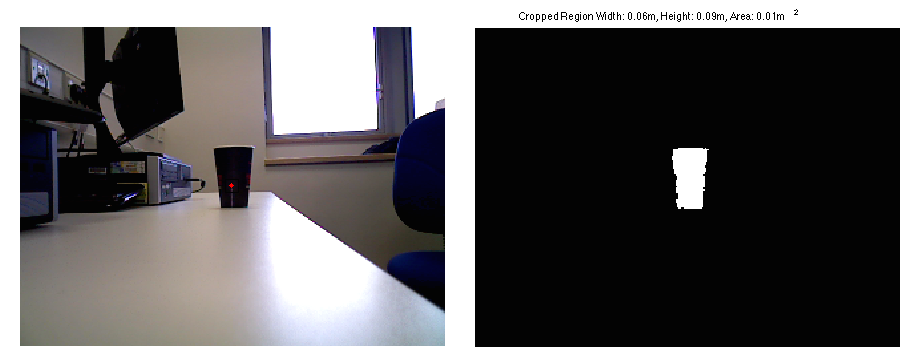
\includegraphics[width=0.8\textwidth]{Navigation/cup.png}
    \caption{Extracted object as a binary image}
\end{figure}

An indicator of the real-terms size of the object was calculated using the following formula:

\begin{equation}
    \mbox{Object Area} = \frac{\sum\limits_x\sum\limits_y \mbox{binaryImage}({x}, {y})}{\mbox{ImageArea}} ({\mbox{FOV}}_{\mbox{width}} \times {\mbox{FOV}}_{\mbox{height}})
\end{equation}

The amplitude of the sine-wave being generated according to the specification in section \ref{sec:centraldistance} was then varied according to the area calculated using the above formula.

\subsubsection{System Performance}

The overhead of having to extract the object from the center of the image reduced the frame processing rate to roughly 14Hz, however this slowdown was barely noticable when using the system

\subsubsection{Effectiveness}
It was proven experimentally that by varying the amplitude of the sound-wave according to the object area, and varying the sound-wave frequency according to the method described in section \ref{sec:centraldistance}, a user could infer both the size of, and the distance to an object. 


\subsection{Multi-point distance}
Building on the method developed in section \ref{sec:centraldistance}, a system able to communicate distance to multiple points simultaneously was also designed.

Rather than simply conveying the distance to the central point in the image, a grid of points was used.

\begin{figure}
    \centering
    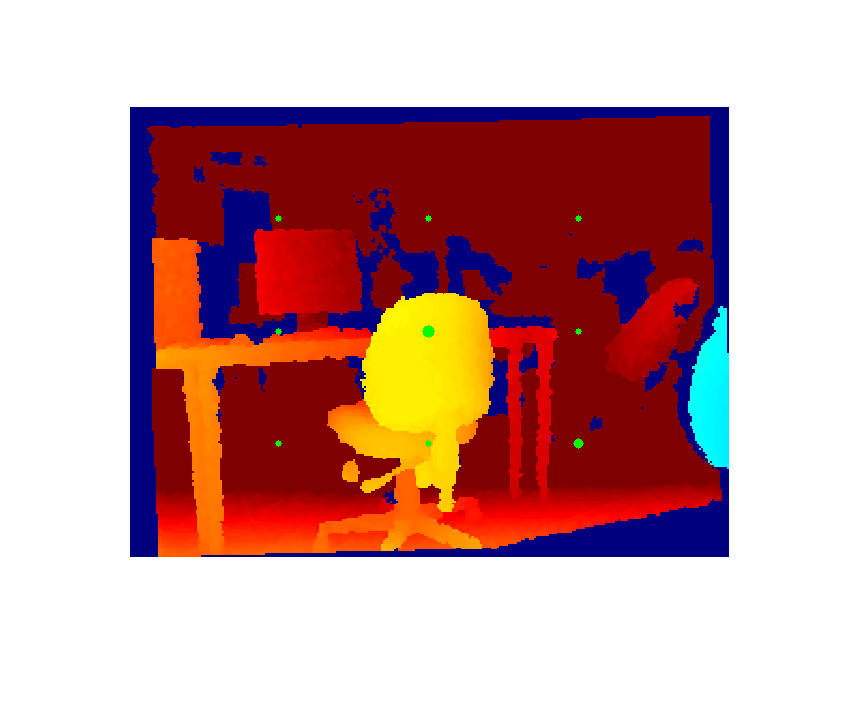
\includegraphics[width=0.5\textwidth]{Navigation/multi-tone.png}
    \caption{Multi-point grid}
\end{figure}

The left column of points was assigned the left stereo channel, the right column was assigned the right stereo channel, with the center column being assigned both stereo channels. 

\section{Shared Components}
\label{sec:sharedcomponents}
\subsection{Magic Wand}
\label{sec:magicwand}
For cases where the object of interest is at a known location in the image, a magic-wand style approach was used for object extraction. 

Searching the Matlab file exchange, a module able to perform magic wand extraction was found\~cite{magicwandmatlab}. The module provides a function, \texttt{magicwand(im, ylist, xlist, tolerance)} that for a given image, set of {x,y} co-ordinates, and a tolerance, creates a mask using the flood-fill algorithm described in section \ref{sec:floodfill}.

\subsection{Tone Generation}
Although Matlab is more than capable of generating and playing back a sine wave, it is not possible to do so while simultaneously performing another task, as it is not possible to write threaded software using normal Matlab syntax. Due to the real-time nature of the system, it was necessary to be able to play back a sine-wave while simultaneously processing video.

In on order to accomplish this, a Java class was developed. This class exposes methods for setting tone frequency, setting tone amplitude and setting pulse duration - internally, a worked tone-generation thread is created. Using this class, it is possible to play back a tone in a non-blocking way. 

Internally, the module uses the \texttt{javax.sound.sampled} package. 

\begin{minted}{java}
BUFFER_SIZE = 2048;
i = 0;
buffer = new byte[BUFFER_SIZE];

while(true){
    samplingInterval = SAMPLE_RATE / getDesiredFrequency();
    angle = (Math.PI*i)/samplingInterval;

    buffer[i%BUFFER_SIZE] = getDesiredAmplitude() * Math.sin(angle);

    if(i%BUFFER_SIZE == 0){
        commitToBuffer();
    }
    i++;
}
    
\end{minted}

Support for pulsing the tone was also implemented. 

\section{Detail Mode}
The development of Detail mode was a much more complicated task than the development of Navigation Mode.

\subsection{Image Segmentation}
Although the primary deliverable of the project was not to invent a new image segmentation algorithm, the method of image segmentation was an important choice.

It was decided that a depth-sensing camera~\cite{xtion} would be used in order to assist with region extraction. Rather than relying solely on RGB data and difference in colour to extract objects from the video footage, depth data would also be considered. This choice was made, as object-segmentation was desired --- if a white cup was placed on a white table, traditional colour-based segmentation algorithms may struggle to differentiate between the object and the surface on which the object was sitting.

As majority of image segmentation algorithm implementations consider only colour information for segmentation; it was not possible to use an off-the-shelf MATLAB module to complete this task. After reviewing publications on segmentation using both depth and RGB data, a few different approaches were trialled.

\subsubsection{Standard Deviation}
As an initial experiment, I attempted to highlight ``interesting'' subsections of the image. This was accomplished by using a sliding window over the RGB image, calculating the standard deviation of the pixels in the window. The resulting image was then thresholded and used on a mask on the original image,

This method was quite successful --- the resulting image only contained objects that stood out on the input image.

\begin{figure}[H]
    \centering
    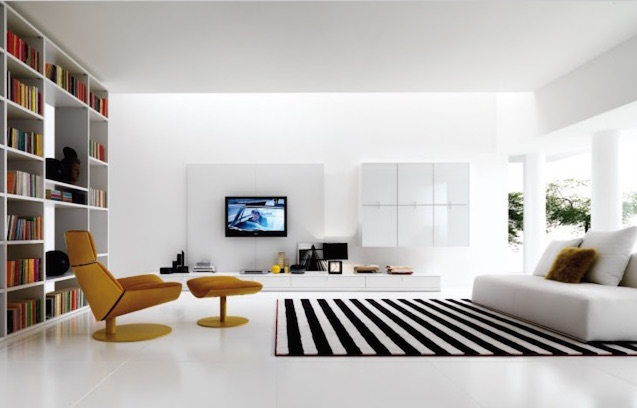
\includegraphics[width=0.6\textwidth]{Segmentation/sd-input.jpg}
    \caption{Input Image}
\end{figure}

\begin{figure}[H]
   \centering
   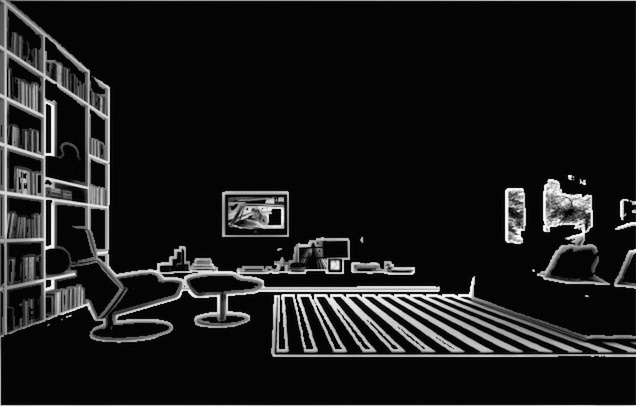
\includegraphics[width=0.6\textwidth]{Segmentation/sd-output.jpg}
   \caption{Standard Deviation Results}

\end{figure}

The main issue with this approach was that Depth Information was not used --- cases where objects had little RGB contrast would not be picked out. 

\subsubsection{K-Means with 4 channels}
One approach was to use a standard K-Means (see section \ref{sec:kmeans}) image segmentation algorithm taken from the Matlab File Exchange~\cite{kmeans-matlab}, with an additional channel added, representing depth. 

\begin{figure}[H]
    \centering
    \begin{subfigure}[b]{0.45\textwidth}
        \centering
        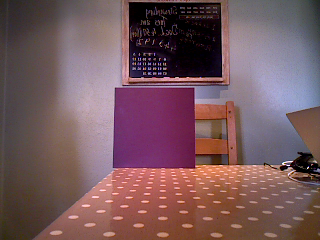
\includegraphics[width=\textwidth]{Segmentation/squarergb-10.png}
        \caption{Input RGB Image}
    \end{subfigure}
    \hfill
    \begin{subfigure}[b]{0.45\textwidth}
        \centering
        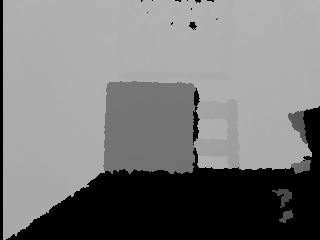
\includegraphics[width=\textwidth]{Segmentation/squaredepth-10.png}
        \caption{Input Depth Map}
    \end{subfigure}
\end{figure}

\begin{figure}[H]
    \centering
    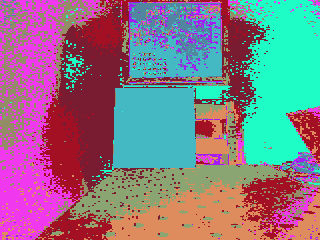
\includegraphics[width=0.4\textwidth]{Segmentation/kmeans-rgb-10seg-im9.png}
    \caption{RGB-only K-Means segmentation}
\end{figure}

\begin{figure}[H]
    \centering
    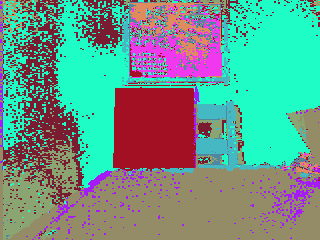
\includegraphics[width=0.4\textwidth]{Segmentation/kmeans-rgb-depth-10seg-im9.png}
    \caption{RGBD K-means segmentation}
\end{figure}

These results were fairly good - the addition of the depth channel resulted in a smoother segmentation. However, using raw images from the camera for segmentation resulted in a fairly noisy image. Applying a Russian blur to the image ($\diameter = 5$, $\sigma = 2$) removed some of the noise, at the expense of sharpness in the image.

\begin{figure}[H]
    \centering
    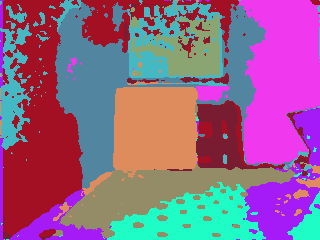
\includegraphics[width=0.4\textwidth]{Segmentation/rgb-depth-kmeans-blurred-10.png}
    \caption{Segmentation of blurred RGBD image}
\end{figure}

Another slight problem with the K-means approach was speed at which it could be performed. While not nearly as slow was some other approaches (such as K-Nearest Neighbour and Graphcuts), performance was limited to the 1-3Hz range.

\subsubsection{K-Nearest Neighbour}


\subsubsection{Channel Swapping}
As mentioned, most segmentation algorithms support only RGB data. With this in mind, another approach taken was to remove a colour channel from the RGB image, and swap it with the depth image. This was quite successful --- the resulting segmentation was more accurate than either RGB or Depth alone.

\subsubsection{Graph Cuts}
Attempts were made to use the Graph Cuts algorithm [REF] in order to segment the video and depth data. However, it became apparent that this approach was taking orders of magnitude longer than we could reasonably spend processing each frame; we wanted the system to run as close to real-time as possible.

\subsection{Conveying Shape Properties}
Two main ways of conveying details about a given shape were considered.

The first, and perhaps most obvious method was to encode and transmit various shape descriptors directly. For instance, the amplitude of a tone of a particular frequency could convey the area of the shape, with a different frequency being used for number of corners, etc etc. This method relies on the shape descriptors being intuitively linked to physical properties of the shape.

The second possible method was to transmit details of a shape in terms of similarity to other ``basis'' shapes.

For instance, consider a method of describing shapes, consisting of 5 parameters. Applying this method to a set of $n$ basis shapes (for instance a circle, square, star and triangle) would yield $n$ sets of 5 parameters. By parametrising an arbitrary shape, and comparing the resulting vector of parameters to the parameter vectors of our basis shapes, it is possible to get a measure of the similarity of our arbitrary shape.

This section of the report details the effectiveness of various methods of conveying different shape properties, using both ``direct encoding'' and basis shape methods.

\subsubsection{Zernike Moments - Direct Encoding}
\paragraph{Direct Encoding}
By assigning a harmonic to each of the Zernike moments, and varying the amplitude of each harmonic according to the moment value, a tone was generated. I then proceeded to pass various shapes into the algorithm, listening to the tone.

\begin{figure}[H]
    \centering
    \begin{subfigure}[h]{0.2\textwidth}
        \centering
        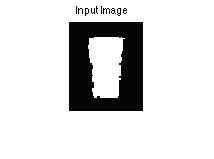
\includegraphics[width=\textwidth]{Detail/zernike-input.png}
        \caption{Input Image}
    \end{subfigure}
    \begin{subfigure}[h]{0.7\textwidth}
        \centering
        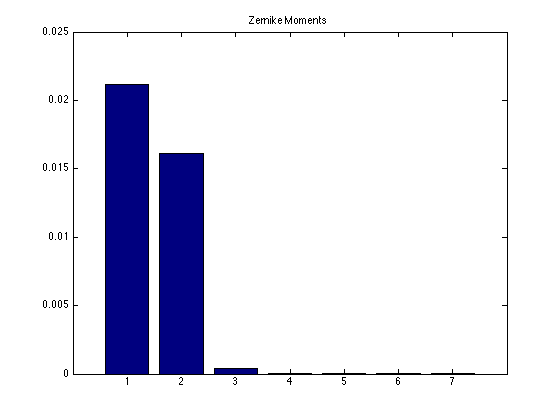
\includegraphics[width=\textwidth]{Detail/zernike-graph.png}
        \caption{Zernike Moments for given input}
    \end{subfigure}
\end{figure}

\begin{figure}[H]
    \centering
    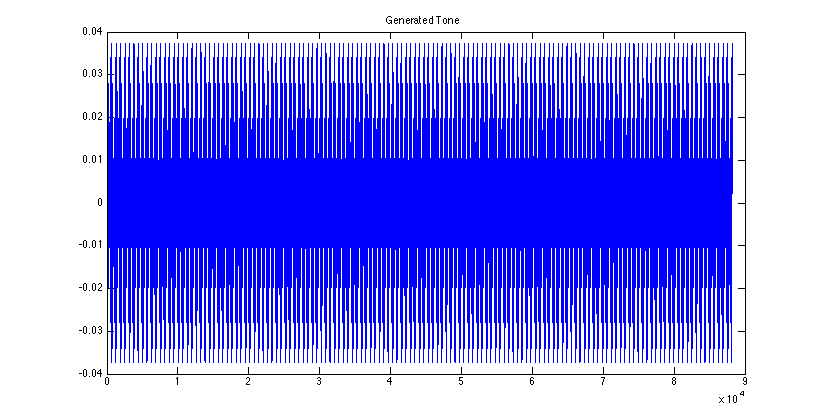
\includegraphics[width=0.8\textwidth]{Detail/zernike-tone.png}
    \caption{Resulting Tone}
\end{figure}

Although the tone varied with each shape, it was not possible to identify individual shapes using this system --- it was unclear how a change in the amplitude of a particular harmonic corresponded to changes in shape.

\paragraph{Zernike Moments - Basis Shapes}

